\documentclass[9pt]{exam} 
\addpoints
\pointsinmargin

\usepackage[fleqn]{amsmath}
\usepackage{amssymb} %standard classy maths symbols
\usepackage[a4paper, margin=1in]{geometry} %makes it easy to specify where to put stuff on the page

\usepackage{tcolorbox} % basic but good package for boxes around text
\tcbset{colback=black!5!white}

\usepackage{tikz, pgfplots} % interval diagrams, sets, etc.
\pgfplotsset{compat=1.18}

\begin{document}

\textbf{Name:} \dotfill

\vspace{-2mm}

\begin{questions}

\question[3] From the definition, find the derivative of $f(x) = \frac{1}{x}$.\newline
\emph{``From the definition" means you must calculate the observable part of $\Delta f / dx$.}

\fillwithdottedlines{48mm}

\question[2] Find the derivative of $g(x) = (x^3 - x) \cdot \sqrt{3}$. \newline
\emph{The question doesn't say ``from the definition" so you can use the formulae on CRM pp. 78-79.}
\fillwithdottedlines{28mm}

\question[2] Determine the equation of the horizontal line $t$ in the sketch below. 
\vspace{-2mm}

\begin{minipage}{0.4\textwidth}
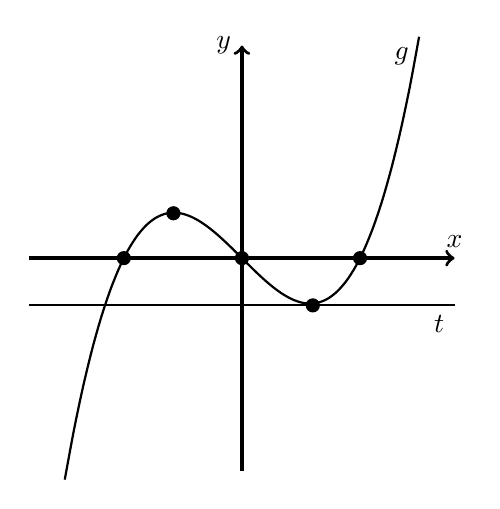
\begin{tikzpicture}[scale=1.5]

\draw[very thick,->] (-1.8,0) -- (1.8,0) node[above] {$x$};
\draw[very thick,->] (0,-1.8) -- (0,1.8) node[left] {$y$};

\draw[domain=-1.5:1.5, samples=40, smooth, thick] plot(\x, {(\x)^3 - \x}) node[below left] {$g$};
\draw[thick] (-1.8,-0.4) -- (1.8,-0.4) node[below left] {$t$};

\fill[black] (0.6, -0.4) circle (0.06);
%\fill[black] (-1.16, -0.4) circle (0.06);

\fill[black] (-1, 0) circle (0.06);
\fill[black] (0, 0) circle (0.06);
\fill[black] (1, 0) circle (0.06);

\fill[black] (-0.58, 0.38) circle (0.06);

\end{tikzpicture}

\end{minipage}
\begin{minipage}{0.6\textwidth}

\fillwithdottedlines{85mm}

\end{minipage}


\vfill

\question[0] \textbf{Bonus.} Find all intercepts and turning points in the sketch. \hfill \emph{Work on the back.}

\question[0] \textbf{Bonus.} Find the coordinates of the other intersection of the curves. \hfill \emph{Polynomial division!}

\end{questions}


\begin{tcolorbox}

\textbf{Name of marker:}

\begin{center}
\gradetable[h][questions]
\end{center}

\end{tcolorbox}


\end{document}